
\chapter{The Standard Model of Particle Physics}
%\section{The Standard Model of Particle Physics}
%
%To pave the way for our future studies we present the SM. Complete with a overview of it's mechanisms and a brief historical introduction.
%
\section{Motivation}

% { \color{red} Note! The motivation should explain why we are going indepth into flavour, and the Yukawa sector. There has to be a purpose to this section! } 

Has stated, it is hard to question the validity of the SM as a successful, at least approximate, framework with whom to describe the phenomenology of Particle Physics up to the largest energy scales probed by collider measurements so far, although some inconsistencies remain and must be addressed.  
%
The SM was proposed in the nineteen sixties by Glashow, Salam and Weinberg and since it has been extensively tested. Both in contemporary direct searches for new physics and indirect probes via e.g. flavour anomalies and precise electroweak parameter measurements in proton-electron collisions. %, { \color{gray} and as said, it's been consistent with most to date.} 

The path to the formulation of the SM came from previous principles relating to symmetries in nature, specifically symmetry in physical laws. 
%
In fact, much in modern physics can be attributed to Emmy Noether's work. She deduced, trough her first theorem, that if the action in a system is invariant under some group of transformations (symmetry), then there exist one or more conserved quantities (constants of motion) which are associated to these transformations. 

Physicist took this idea and were led to the fundamental question behind the SM, is it possible that upon imposing to a given Lagrangian the invariance under a certain group of symmetries to reach a given form for it's the dynamics? 
%
These dynamics would be in our context, particle interactions. This train of thought first led to Quantum Electrodynamics (QED), then Quantum Chromodynamics (QCD) and finally the SM. 
%
We can quote Salam and Ward: % A. Salam and J. C. Ward, Nuovo Cim.19, 165 (1961). 

\textit{“Our basic postulate is that it should be possible to generate strong,  weak and electromagnetic  interaction terms (with all their correct symmetry properties and also with clues regarding their relative strengths) by making local gauge transformations on the kinetic energy terms in the free Lagrangian for all particles.”}

We are glossing over a lot of complexity here, and for the SM to be properly formulated additional concepts would be required. In the case of weak interactions, the presence of very heavy weak gauge bosons require the new concept of spontaneous breakdown of the gauge symmetry and the Higgs mechanism \cite{higgs1964broken,englert1964broken,guralnik1964global} . 
%
While the concept of asymptotic freedom played a crucial role to describe perturbatively the strong interaction at short distances \cite{politzer1973reliable,gross1973ultraviolet}.  

\renewcommand{\cleardoublepage}{}
\renewcommand{\clearpage}{}

\section{Internal symmetry of the Standard Model}
%
The SM is a "standard" QFT gauge theory, that is to say, it is manifestly invariant under a set of field transformations. The SM gauge group, $\mathcal{G}_{SM}$, is seen in, 
%
\begin{equation}
\mathcal{G}_{SM} = \mathrm{SU}(3)_{\mathrm{c}} \times \SU{L} \times \U{Y} \quad  .
\label{eq:SM_Group}
\end{equation} 
%
Here we have, first, the $\mathrm{SU}(3)_{\mathrm{c}}$ group corresponding to quantum chromodynamics (QCD), responsible for the strong force, this symmetry will remain unbroken by the electroweak VEV. Secondly, we have the $\SU{L} \times \U{Y}$ portion that will be broken by the Higgs mechanism into $\U{Q}$, the electromagnetic gauge symmetry.
%
Each particle stems from a field that is charged in a particular manner on each of these groups, making the charge triplets we will come to later define. 
%
Given the invariance under the group in eq.\,\ref{eq:SM_Group}, it is impossible have any field that is charged have a explicit mass term. This chapter will focus on how the mass of particles is generate trough the Higgs mechanism. And offer a brief discussion of flavour physics in the SM and how flavour changing currents can point to {\color{blue} New Physics (NP)}. 

%{ \color{gray} All masses for the fermions and leptons are generated trough their interactions with the Higgs Boson. This mass generation as the Higgs Boson settles into it's VEV is called the Higgs Mechanism. } 

\subsubsection{Gauge Group numbers}

The full set of quantum numbers in all the SMs fields are described in the tables \ref{table1} and \ref{table2}, this is their color charge, weak isospin number and the hypercharge, written in that order as entries in each triplet.
%
\begin{table}[H]
\centering
\caption{Gauge and Scalar fields dimensions in the SM}
\label{table1}
\begin{tabular}{@{}cccccc@{}}
  \hline	
 Fields & Spin 0 field & Spin 1 Field & $SU(3)_C \times SU(2)_L \times U(1)_Y$  \\
  \hline	
 Gluons  & $\times$  & $g$ & (8,1,0) \\	
A bosons & $\times$  & $A^i$ & (1,3,0)   \\
B bosons & $\times$  & $B$ & (1,1,0)   \\
Higgs field & ($\phi^\pm, \phi^0 )$  & $\times$ & (1,2,1) \\ \hline
\end{tabular}
\end{table}
%
\begin{table}[H]
\centering
\caption{Fermion field dimensions in the SM}
\label{table2}
\begin{tabular}{@{}cccccc@{}}
  \hline	
 Fields & Spin $\frac{1}{2}$ Field & $SU(3)_C \times SU(2)_L \times U(1)_Y$  \\
  \hline	
Quarks (3 gen.) & $Q=(u_L,d_L)$ & $(3,2,\frac{1}{3})$ \\	
$\quad$        & $u_R$ & $(3,1,\frac{4}{3})$   \\
$\quad$   & $d_R$ & $(3,1, -\frac{2}{3})$   \\
Leptons (3 gen.) & $(L=(\nu_{e_L}, e_L )$ & $(1,2,-1)$  \\
$\quad$   & $e_R$ & $(1,1,-2)   $ \\ \hline
%
\end{tabular}
\end{table}
%
From here, given the gauge group in, eq.\,\ref{eq:SM_Group} and accounting for the charges and fields, we can derive the form of the SM's Lagrangian. These gauge groups are composed of 12 generators and are governed by the following algebra, 
% 
\begin{equation}
\left[ L_a , L_b \right] = i f_{abc} L_c \quad \left[ T_a , T_b \right] = 1 \epsilon_{abc} T_c \quad \left[ L_a , T_b \right] = \left[ L_a , Y \right] = \left[ T_b,Y \right] = 0 
\end{equation}
%
where for the $\mathrm{SU(3)_c}$ triplets, $L_a= \frac{\lambda_a}{2}$ , $(a = 1, . . . , 8)$ {\color{gray} contrary to $\mathrm{SU(3)_c}$ singlets where, $L_a = 0$}.  As for the $\mathrm{SU(2)_L}$, we have $T_i= \frac{\sigma_i}{2} $, $(i = 1, 2, 3)$, {\color{gray} being that again for singlets $T_b=0$}. $Y$ is the generator of $U(1)_Y$. The symbols $\lambda_a$ and $\sigma_i$ represent the Gell-Mann and Pauli matrices respectively. 

\subsection{Fields, Particles and Lagrangian of the SM}

From these fields the physical states of the SM, it's particle spectrum, is composed by, first, the gauge bosons, the weak force carriers, $W^\pm$ and $Z$ bosons, and the photon $\gamma$, the electromagnetic interaction messenger and the strong force mediators, the gluons, $g$, as well, of course, by the matter particles, the fermions, composed by the quarks and leptons. 

Leptons and quarks are organized in three generations each, with 2 pairs by each generation leading to 6 different particles for each. 
%
For quarks we have the up and down for the first generation, charm and strange for the second as well as top and bottom for the third one. 
%
Similarly, there are 6 types of leptons, the charged ones, electron, muon and tau, and the associated neutrinos. These are represented in different manners, being that the quarks are represented by the letters $(u,d,c,s,t,b)$ while leptons as $(e,\nu_{e},\mu,\nu_{\mu},\tau,\nu_{\tau})$. 

Fermions are half integer spin particles half of which have electrical charge (except the neutrinos).  While quarks interact via the weak, electromagnetic and strong forces, the charged leptons only feel the electromagnetic and weak forces and the neutrinos are weakly interacting.  
%
A physical fermion is composed of a left-handed and a right-handed field. While the left transform as $SU(2)_L$ doublets and can be written as,
%
\begin{equation}
L^i= \begin{pmatrix}
\nu_{e_L} \\ e_L 
\end{pmatrix},
\begin{pmatrix}
\nu_{\mu_L} \\ \mu_L 
\end{pmatrix},
\begin{pmatrix}
\nu_{\tau_L} \\ \tau_L 
\end{pmatrix} 
\quad 
\text{and} \quad Q^i= \begin{pmatrix}
u_{L} \\
d_L 
\end{pmatrix},\begin{pmatrix}
c_{L} \\
s_L 
\end{pmatrix}
,\begin{pmatrix}
t_{L} \\
b_L 
\end{pmatrix} \quad ,
\end{equation}
where the $i$ index stands for generation, often designed as the flavour index, the latter are $\SU{L}$ singlets and can be simply represented as
%
 \begin{equation}
e^i_R=\{e_R,\mu_R,\tau_R\}, \quad  u^i_R=\{u_R,c_R,t_R\}, \quad d^i_R=\{d_{e_R},s_{e_R},b_{e_R}\} \quad , 
\end{equation}
%
note also that the quarks form triplets of $\mathrm{SU(3)_C}$ whereas leptons are colour singlets. The Higgs boson also emerges from an $\mathrm{SU(2)_L}$ doublet with the form,
%
\begin{equation}
H=\begin{pmatrix}
\phi^1 + \; i \; \phi^2 \\
\phi^3 + \; i \; \phi^4  
\end{pmatrix} \quad , 
\end{equation}
%
%The Lagrangian that describes all vector particles and gauge fields in the SM can be writen as
%
Here we see the four components that correspond to the respective degrees of freedom of the Higgs Field.
% 
After the process of SSB of the $\mathrm{SU(2)_L} \times \U{Y}$ group the charges of the fermions along their QCD and QED numbers become, 
%
\begin{table}[H]
\caption{Quark and Lepton charges}
\centering
\begin{tabular}{ccc}
  \hline & $\mathrm{SU(3)_C}$ & $\mathrm{U(1)_Q}$ \\
  \hline 
Up type quarks $(u,c,t)$ & 3 & 2/3 \\
Down type quarks $(d,s,b)$ & 3 & -1/3 \\
Charged leptons $(e,\mu,\tau)$ & 1 & -1 \\
Neutrinos  $(\nu_e,\nu_\mu,\nu_\tau)$  & 1 & 0 \\
  \hline	
\end{tabular}
\end{table}

\subsubsection{Lagrangian formulation }
%
Given the SM gauge groups and charges seen in \ref{eq:SM_Group} the covariant derivative, $D_\mu$, will read as, 
%
\begin{equation}
\label{eq:PartialDefSM}
D_\mu = \partial_\mu - i g_S \tau^a G^a_\mu - i g T^i A^i_\mu - i g' Y B_\mu \quad ,  
\end{equation}  
%
We can expect 3 different type of couplings, $g_s$ related to the $\mathrm{SU(3)_C}$ subgroup, $g$ to the $\mathrm{SU(2)_L}$ and $g^\prime$ to $\mathrm{U(3)_Y}$. The associated canonical field strength tensors would be,
\begin{align}
G_a^{\mu \nu} & = \partial^\mu G^\nu_a - \partial G^\mu_a - g_s f_{abc} G_a^\mu G_b^\nu  \\ 
A_a^{\mu \nu} & = \partial^\mu A^\nu_a - \partial^\nu A^\mu_a  - g \epsilon_{abc} A^\mu_b A^\nu_c \\
B^{\mu \nu}   & = \partial^\mu B^\nu - \partial^\nu B^\mu 
\end{align}
It is often convenient to present the SMs Lagrangian in portions, usually divided in three sections,
\begin{equation}
\mathcal{L}_{SM} = \mathcal{L}_{kin}  +  \mathcal{L}_{Yuk} +  \mathcal{L}_{\phi} 	
\end{equation}
Where we have the kinetic portion of the SM terms,$\mathcal{L}_{kin}$, responsible for  free propagation of particles, the Yukawa portion, $\mathcal{L}_{Yuk}$  corresponding to interactions of particles with the Higgs Boson, and finally the $\mathcal{L}_{\phi}$ scalar potential. The full kinetic portion of the SM read, 
%
\begin{align}
\label{eq:KinSM}
\mathcal{L}_{kin} = & - \frac{1}{4} G^{\nu \mu}_a G_{a \,\nu \mu}  - \frac{1}{4}  A^{\nu \mu}_a A_{a \,\nu \mu}  
- \frac{1}{4}  B^{\nu \mu} B_{\nu \mu} \nonumber \\ 
 & -i \overline{Q_{L_i}} \slashed{D} Q_{L_i} 
   -i \overline{u_{R_i}} \slashed{D} u_{R_i}  
   -i \overline{d_{R_i}} \slashed{D} d_{R_i}  
   -i \overline{L_{L_i}} \slashed{D} L_{L_i}    
   -i \overline{e_{R_i}} \slashed{D} e_{R_i}   \\
 & - (D_\mu H)^\dagger ( D^\mu H )   \nonumber 
\end{align}
Where $\slashed{D}$ is the Dirac covariant derivative, $\gamma^\mu D_\mu$. { \color{gray} From the last line Eq.\,\ref{eq:KinSM} and with Eq.\,\ref{eq:PartialDefSM} we will present how the Generators $A^i_\mu$ and $B_\mu$ give rise to the weakly interacting vector bosons $W^\pm$ and $Z^0$ and the electromagnetic vector boson $\gamma$. Contrary to the color sector, where the eight generators $G^a_\mu$ simply correspond to eight gluons $g$ a mediating strong interactions. } { \color{blue} Maybe move this to where it actually is written } 
%
While the scalar potential part 
%
\begin{equation}
\mathcal{L}_{\phi} = -\mu^2 H H^\dagger - \lambda (H H^\dagger)^2
\end{equation}
Finally the Yukawa portion of the Lagrangian would be written as, 
\begin{equation}
\label{eq:YukawaSM}
\mathcal{L}_{Yuk} = Y^u_{ij} \overline{Q_{L_i}} u_{R_j}  \tilde{H} + Y^d_{ij} \overline{Q_{L_i}}  d_{R_j} H  + Y^e_ij \overline{L_{L_i}}  e_{R_i} H + h.c. 
\end{equation}
%
Here we have, $\tilde{H}=i\sigma_2 H$.
%
{ \color{gray} It is due to the Yukawa interactions between the Higgs and the fermions and leptons that these acquire their masses once the Higgs settles into his VEV. } { \color{blue} same as before }

\renewcommand{\cleardoublepage}{}
\renewcommand{\clearpage}{}

\section{The Higgs mechanism and the mass generation of the Gauge bosons}

From what was defined above, we can now study the process SSB by which, 
%
\begin{equation}
\SU{L}\times\U{Y} \rightarrow \U{Q}
\end{equation} 
%
and carry trough to the Higgs Mechanism. Enabling us to find the real physical states of the gauge bosons and the origin of their mass. Let us then consider the part of the Lagrangian containing the scalar covariant derivatives, the scalar potential and the gauge-kinetic terms:
%
\begin{equation}
\mathcal{L}_{Gauge} \supset (D_\mu H)(D^\mu H)^\dagger - \mu^2 H^\dagger H - \lambda (H^\dagger H)^2 - \frac{1}{4}  W^{\nu \mu}_a W_{a \,\nu \mu}  
- \frac{1}{4}  B^{\nu \mu} B_{\nu \mu}
\label{eq:GaugeSM}
\end{equation} 
% 
We expect a phase shift to occur, namely one that ensures $\mu^2 < 0$ while at the same ensuring that the field now explicitly breaks the $\mathrm{SU(2)_L \times U(1)_Y}$. For this to happen we expect the shifted squared value of the Higgs field to be,
%
\begin{equation}
(H^\dagger H) = \frac{-\mu^2}{2\lambda} = \frac{1}{2} v  \quad , 
\end{equation} 
This VEV, called the electroweak VEV, is experimentally measured to be $v \approx 246$ GeV. 
%
The choice of vacuum can be aligned in such a way that we have,
\begin{equation}
H_{min} = \frac{1}{\sqrt{2}} \begin{pmatrix} 0 \\
v 
\end{pmatrix} \quad .
\end{equation}

Given that now the $SU(2)_L \times U(1)_Y$ symmetry is broken down to $U(1)_Q$ we jump from a scenario where there were four generators, which are $T^{1,2,3}$ and $Y$, to, after the breaking, having solely one unbroken combination that is $Q =  (T^3 + 1/2)$ associated to the electric charge. This means that in total we will have three broken generators, thus, from Goldstone Theorem, there would have to be created three massless particles. 

These Goldstones modes however can then be parametrized as phases in the field space and then can be "rotated away" in the physical basis, leaving us with a single physical massive scalar, the Higgs boson. Note that, with this transformation we are removing three scalar degrees of freedom.  However, they cannot just disappear from the theory and will be absorbed by the massive gauge bosons.
%
In fact, a massless gauge boson contains only two scalar degrees of freedom (transverse and polarization). Meanwhile, a massive vector boson has two transverse and a longitudinal polarization, i.e., three scalar degrees of freedom. So, as we discussed above, while before the breaking of the EW symmetry we have four massless gauge bosons, after the breaking we are left with three massive ones. This means that there are three extra scalar degrees of freedom showing up in the gauge sector. It is then commonly said that the goldstone bosons are ``eaten" by the massive gauge bosons and the total number of scalar degrees of freedom in the theory is preserved. Therefore, without loss of generality, we can rewrite the Higgs doublet as
%
\begin{equation}
 \begin{pmatrix}
G_1 + i G_2 \\ 
v + h(x) + i G_3 
\end{pmatrix} = H (x) \rightarrow H (x) =  \frac{1}{\sqrt{2}} \begin{pmatrix}
0 \\ 
v + h(x) 
\end{pmatrix} \quad .
\label{shame}
\end{equation}
Once the Higgs doublet acquires a VEV, the Lagrangian (\ref{eq:GaugeSM}}) can be recast as:
%
\begin{align}
\mathcal{L}^\prime = & \frac{1}{2} \partial_\mu h \partial^\mu h - \frac{1}{2} (2v^2 \lambda) h^2
 - \frac{1}{4}  W^{\nu \mu}_a W_{a \,\nu \mu}  
- \frac{1}{4}  B^{\nu \mu} B_{\nu \mu}  \nonumber \\
& + \frac{1}{8} v^2 g^2 (A^1_\mu A^{1,\mu}+ A^2_\mu A^{2,\mu}) +  \frac{1}{8} v^2  (g^2  A^3_\mu A^{3,\mu} + g^{\prime 2} B_\mu B^\mu - 2 g^2 g^{\prime 2} A^3_\mu B^\mu ) \quad , 
\label{complicatedpart}
\end{align}
%
A few things become obvious first, we have a lot of mass terms most stemming from the squared gauge fields and a lonesome squared mass term belonging to the real scalar field we know to be the Higgs field. This makes the Higgs boson mass in the SM to be given by,
%
\begin{equation}
M_h= (2v^2 \lambda) \quad .  
\end{equation}
%
To obtain masses for the gauge bosons we need to rotate the gauge fields to a basis where the mass terms are diagonal. First, it is straightforward to see that the electrically charged eigenstates are given by %\ref{gagestate}
%First the fields that carry defined charge that can be easily shown to be 
\begin{equation}
W^\pm_\mu = \frac{1}{\sqrt{2}} (A^{(1)}_\mu \pm i A^{(2)}_\mu) \quad , 
\label{gagestate}
\end{equation}
meaning that the mass of the W bosons is, 
\begin{equation}
M_{W^\pm}= \frac{1}{2} v g \quad .
\end{equation}
%
The situation becomes a bit more complicated for the second term in (\ref{complicatedpart}) due to a mixing between $A_\mu^3$ and $B_\mu$. In the gauge eigenbasis the mass terms read
%
\begin{equation}
\begin{pmatrix}
A_\mu^3 && B_\mu
\end{pmatrix} \cdot  \frac{1}{4} \nu ^2 \begin{pmatrix}
g^2  & -g g^\prime \\
-g g^\prime & g^{\prime 2} 
\end{pmatrix} \cdot \begin{pmatrix}
A_\mu^3 \\  B_\mu
\end{pmatrix}  \quad , 
\end{equation} 
%
which can be diagonalized to obtain,
%
\begin{equation}
\begin{pmatrix}
A_\mu && Z_\mu 
\end{pmatrix} \begin{pmatrix}
0  & 0 \\
0  & \frac{1}{2} v \sqrt{g^2 + g^{\prime 2}} 
\end{pmatrix}  \begin{pmatrix}
A^\mu \\ Z^\mu
\end{pmatrix}  \quad , 
\end{equation}
%Where the new eigenvectors that represent the $Z$ boson and the photon, $A^\mu$ in terms of the former base are written as,
%
we identify the eigenvector associated to the eigenvalue 0 to the photon and the massive one, $ M_Z =  \frac{1}{2} v \sqrt{g^2 + g^{\prime 2}} $, to the Z boson. Such eigenvectors can be written as
%
\begin{align}
A_\mu &=\cos(\theta_\omega) B_\mu + \sin(\theta_\omega) A_\mu^3 \quad ,  \\  
Z_\mu & =- \sin(\theta_\omega) B_\mu + \cos(\theta_\omega) A_\mu^3 \quad , 
\end{align}
%
where $\theta_w$ is the so called Weinberg mixing angle and is defined as, 
%
\begin{equation}
\cos(\theta_\omega)=\frac{g}{ \sqrt{g^2 + g^{\prime 2}}} \quad ,  
\end{equation}
%
thus clearly showing the massless photon along with a massive Z boson with mass $M_Z= \frac{1}{2} \nu \sqrt{g^2 + g^{\prime 2}} $. 
%
So we conclude our exploration of the electroweak sector with all the correct massive spectrum observed and its origin discussed.

\renewcommand{\cleardoublepage}{}
\renewcommand{\clearpage}{}

\section{Fermion Masses in the SM and Quark mixing}

As referenced \Joaoadd{previously}, given the charges of the fermion and lepton fields\Joaoadd{,} we cannot construct a gauge invariant theory with explicit mass terms for fermions. 
%
The mass of these particles \Joaorep{are generated through couplings to the Higgs, by the Higgs mechanism}{are generated through the Higgs mechanism, via Yukawa terms between the fermions and the scalar field. These interactions can be seen in Eq.\,\eqref{eq:YukawaSM}}. \Joaoout{We can write these interactions as,}
%
%\begin{equation} 
%\label{eq:Yukawa2}
%\mathcal{L}_{Yuk} = Y^u_{ij}\bar{Q}_{i} u_{R_j}  \tilde{H} + Y^d_{ij} \bar{Q}_{i}  d_{R_j} H  + Y^e_{ij} \overline{L_{L_i}}  e_{R_i} H + h.c.
%\end{equation} 
%
\Joaoout{where $Y^{e,u,d}$ stand for the Yukawa matrices, these are generic $3\times3$ complex non-dimensional coupling matrices, $H$ is the Higgs field with $\tilde{H}$ retaining it's previous definition, $i,j$ are the standard generation indices, $Q_{L_i}$,are the left handed quark doublets, while $d_R$ and $u_R$ are the corresponding right-handed down and up quark singlets respectively in the weak eigenstate basis.}
%
\Joaorep{Has}{As} the Higgs field settles into the electroweak VEV \Joaoadd{(see Eq.\,\eqref{eq:vev_expansion})} \Joaoout{yields} mass terms for the quarks and leptons \Joaoadd{are generated}. 
%
The Higgs mechanism generates the mass for all the fermionic and leptonic particles except for neutrinos\Joaoadd{. T}his is due to the SM not containing right handed neutrinos, i.e we \Joaorep{can't}{can not} build terms that would lead to neutrino masses.
% 
The addition of right handed neutrino fields is very commonly made in BSM scenarios. 

To reach the physical states \Joaoout{starting} from the weak eigenbasis \Joaorep{you}{we} must diagonali\Joaoadd{s}e the Yukawa matrices. This is done through \Joaoout{a} bi-unitary transformation\Joaoadd{s}. 
% 
We can write these transformation under the form,
%
\begin{equation}
\label{YukawaMasses} 
M^{u,d,e}_{\text{diag.}}= U^{u,d,e}_L Y^{u,d,e} U^{u,d,e}_R 
\end{equation} 
%
\Joaorep{where $v$ stands for the electroweak VEV. And}{where} $U^{u,d,e}_L$ and $U^{u,d,e}_R$ are \Joaoout{the required} \Joaorep{6}{4} unitary matrices. \Joaoadd{For simplicity, we shall assume that in the leptonic sector the Yukawa matrices are flavour diagonal, hence, only the two unitary matrices for the quarks will be of relevance to our discussing bellow.}
%
\Joaoout{
It is, in fact, these matrices that will get us from the flavour eigenbase to the mass eigenbase. }
%
%{\color{gray} The charged lepton Yukawa matrix can always be made real and positive through a bi-unitarity transformation.  
%
%Meaning the Yukawa matrix for the leptons contains only 3 real physical parameters that correspond to the Lepton masses. } 
%
Naturally\Joaoadd{,} we can invert Eq.\,\eqref{YukawaMasses}, returning \Joaoout{equations for the Yukawa matrices as,} 
\begin{equation}\label{eq:YukawaBiUni}
\begin{aligned}
Y^u_{ij} = &  (U_L^u M^u_{\text{diag.}} U_R^u)_{ij}, \\
Y^d_{ij} = &  (U_L^d M^d_{\text{diag.}} U_R^d)_{ij}.
\end{aligned}
\end{equation}
%
\Joaoadd{Considering now the Higgs mechanism,} we can see this change creates mass terms for physical quark fields by replacing the result of Eq.\,\eqref{eq:YukawaBiUni} in the Yukawa portion of the Lagrangian Eq.\,\eqref{eq:YukawaSM}
%
\begin{gather}
\mathcal{L}_{Yuk} \supset 
- Y^d_{ij} \begin{pmatrix} \overline{u}_{L\,i} & \overline{d}_{L\,i}  \end{pmatrix}  d_{R\,j} \Joaoadd{\tilde{H}} 
%
- Y^u_{ij} \begin{pmatrix} \overline{u}_{L\,i} & \overline{d}_{L\,i}  \end{pmatrix} \, u_{R\,j} H + \Joaoadd{\mathrm{H.c.}} \nonumber  \\ 
% % % 
 \Downarrow \nonumber \\
-(U_L^d m^d_{\text{diag.}} U_R^d)_{ij} d_{L\,i} \, d_{R\,j}  - (U_L^u m^u_{\text{diag.}} U_R^u)_{ij} u_{L\,i} \, u_{R\,j} + \big(\text{Interactions \Joaoadd{with $h$}}\big) + \Joaoadd{\mathrm{H.c.}} \\ 
 \Downarrow  \nonumber \\ 
-m^d_{\text{diag.}_j} d_{L\,i}^\prime \, d_{R\,j}^\prime  - m^u_{\text{diag.}_j} u_{L\,i}^\prime \, u_{R\,j}^\prime + \big(\text{Interactions \Joaoadd{with $h$}}\big) + \Joaoadd{\mathrm{H.c.}}  \nonumber  
\end{gather}
%
\Joao{Hermitian é em homenagem ao matemático Charles Hermite, portanto tem que estar em maiúsculo, H.c. e não h.c.} where the primed fields are the quark fields in the mass basis, defined as 
\begin{equation}
\begin{split}
d^\prime_{L,R} = U^d_{L,R} d_{L,R}, \\
u^\prime_{L,R} = U^u_{L,R} u_{L,R}.
\end{split}  
\end{equation}
% 
Note that the increasing masses seen in each generation depend directly on the \Joaoout{term} hierarchy of the Yukawa terms. This means that the mass of all particles directly relate\Joaoadd{s} to how strongly they each interact with the Higgs boson.
%
If you then take into account the real masses e.g. for the leptons, the tau mass is in the GeV range while the electron's is in the 0.1 MeV range. \Joaorep{These translate}{This translates} to very different couplings for each flavour. 
%
This hierarchy is unjustified in the SM. 

As a result of this redefinition, we can now look at the gauge interactions to see that \Joaoout{a} charge\Joaoadd{d} current\Joaoadd{s} appear\Joaoout{s} where $W^\pm$ couples \Joaoadd{to} the physical $u^\prime_{L_j}$ and $d^\prime_{L_j}$ \Joaoadd{quarks}. 
%
The coupling of the \Joaoout{of} fermions to \Joaorep{their respective}{the} gauge fields changes by virtue of the fact \Joaoadd{that} only left handed \Joaoadd{q}uarks are $\mathrm{SU(2)_L}$ doublets\Joaoadd{. I}f we expand the up and down quark fields on the kinetic portion of the Lagrangian
%
\begin{equation}\label{LagFermFCCCs}
\begin{aligned}
\mathcal{L}_{ferm} \supset & 
\frac{1}{2} \Joaoadd{\bar{u}}^\prime_L \gamma^\mu \left( g^\prime \Joaoadd{Y} B_\mu + g \Joaoadd{Z}_\mu  \right) \left(U^u_L U^{u \dagger}_L \right) u^\prime_L - \frac{1}{\sqrt{2}} g \Joaoadd{\bar{u}}^\prime_L \gamma^\mu \left( U^u_L U^{d \dagger}_L \right) d^\prime_L W^+_\mu \\   
- 
& \frac{1}{\sqrt{2}} g \Joaoadd{\bar{d}}^\prime_L \gamma^\mu \left( U^u_L U^{d \dagger}_L \right) u^\prime_L W^-_\mu 
+ 
\frac{1}{2} \Joaoadd{\bar{d}}^\prime_L \gamma^\mu \left( g^\prime \Joaoadd{Y} B_\mu - g \Joaoadd{Z}_\mu \right) \left( U^d_L U^{d \dagger}_L \right) d^\prime_L.  
\end{aligned}
\end{equation}
%
\Joaorep{We can trough the use of the properties of unitary matrices}{By employing properties of unitary matrices}, namely, $ \mathrm{U}^{u,d}_{L,R} \mathrm{U}^{u,d \dagger}_{L,R} = 1$, \Joaoadd{we} note that the interactions with the neutral bosons remain the same in the mass basis.
%
However the charged currents are affected by this change.
%
Therefor, we define the Cabibbo-Kobayashi-Maskawa (CKM) matrix, as $V_{CKM} = U^u_L U^{u ^\dagger }_R $ and write the sensitive terms,
%
\begin{equation}
\mathcal{L}_{kin} \supset \frac{1}{\sqrt{2}} g \overline{u}^\prime_L \gamma^\mu V_{CKM} d_L^\prime W^+_\mu + h.c. 
\end{equation}
%
The CKM matrix, is a $3 \times 3$ unitary matrix. It is a parametrization of the three mixing angles and CP-violating KM phase. There are many possible conventions to represent the CKM matrix.\Joao{Ref. Secalhar o PDG, que eles têm uma secção dedicada a isto das diferentes convenções e fases.}
%
The mixing angles refer to those between the up and down quark families. We can see their hierarchy in Fig. \ref{fig:QuarkCKM}.

It is through this complex phase in the CKM matrix that the SM can account for the phenomena of $\mathcal{CP}$ violation. First observed in the famous $K^0$ decay into $\mu^+$ $\mu^-$ ($CP=+1$ and $CP=-1$ respectively\Joaoadd{, see Fig.~\ref{fig:Kaon}}) that won the 1980 Nobel Prize \Joao{Ref}. The discovery opened the door to questions still at the core of particle physics and of cosmology today \Joao{Esta frase não soa bem, acho melhor que a reescrevas}. Not just the lack of an exact CP-symmetry, but also the fact that it is so close to a symmetry. {\color{blue} citation}

\begin{figure}[H]
	\centering
	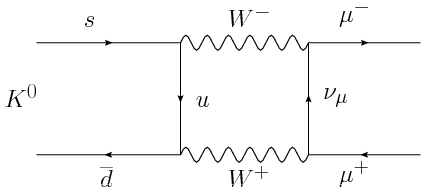
\includegraphics[width=0.5\textwidth]{Glashow-Illiopoulos-Maiani_mechanism_fig1.png}
	\caption{Box diagram describing $K_L^0\rightarrow\mu^-\mu^+$, through an intermediate $u$ quark. \Joao{A imagem tem pouca qualidade. Consegues fazer isto no latex com a package feynmp. No tutorial que te enviei tem lá o código}}
	\label{fig:Kaon}
\end{figure}

\Joaoout{We avoided discussing leptons since in the SM their mass eigenstates can be easily shown to have no real consequence besides a change of basis.} 
%
\Joaorep{You}{We} might also note a very interesting feature of the Standard Model, by consequence of the $\mathrm{SU(2)_L \times U(1)_Y }$ symmetry\Joaoadd{. T}here are no interactions of the right handed unitary matrices and \Joaorep{there for}{thus} no mixing, coupling, or charged currents of right handed quarks, making them theoretically invisible to measurements. \Joao{Já notei que às vezes usas ``you''. Não te dirigas para o arguente ou para que está a ler. Tenta usas sempre expressões com ``We''}
%
\begin{figure}[H]
	\centering
	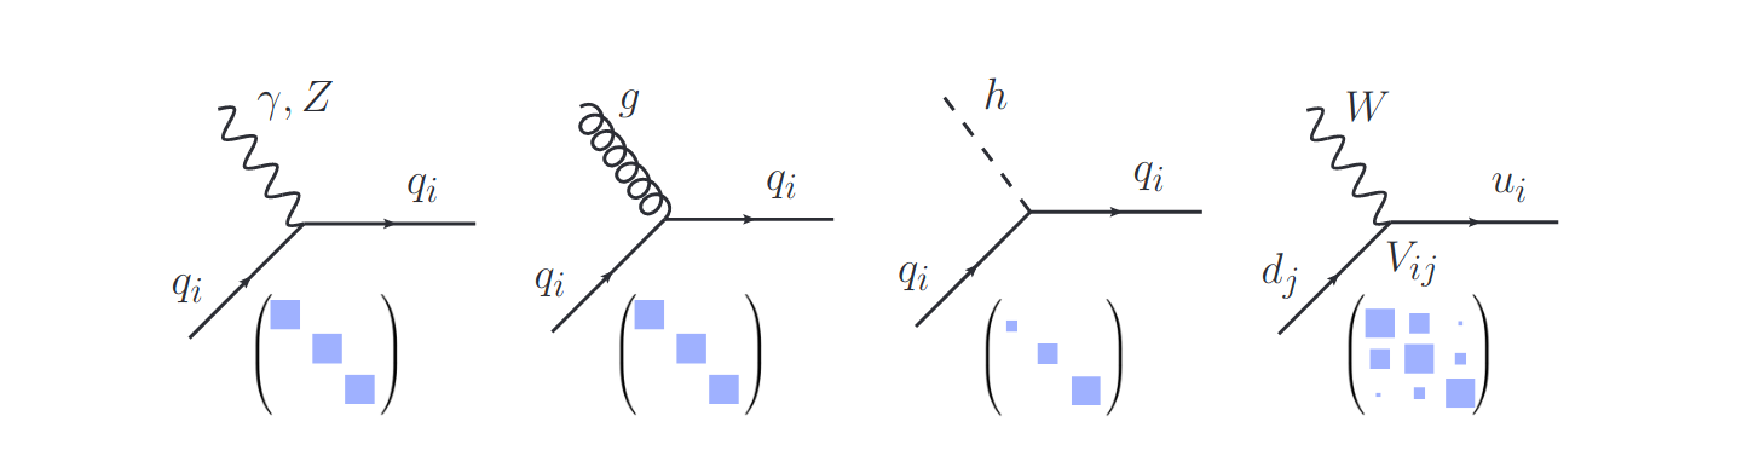
\includegraphics[width=0.9\textwidth]{TestYukawaCouplings.pdf}
	\caption{\Joaoout{The} Feynman diagrams for flavour conserving couplings of quarks to photon, $Z$ boson, gluon and the Higgs (the first three diagrams), and the flavour changing coupling to the $W$ (the last diagram). The $3\times3$ matrices are visual representations of couplings in the generation space, with couplings to $\gamma$, $Z$, $g$ \Joaoadd{being} flavour universal, \Joaorep{the}{while} couplings to the Higgs flavour \Joaoadd{are} diagonal but not universal\Joaorep{, and the couplings to}{. The couplings involving} $W$ \Joaoadd{are} flavour changing and hierarchical.}
	\label{fig:QuarkCKM}
\end{figure}
%

% Possible power gap
%
% Here we introduce the CKM matrix, a $3 \times 3$ unitary matrix. It is a paramatrization of the three mixing angles and CP-violating KM phase. There are many possible conventions to represent the CKM matrix. 

The CKM matrix elements are fundamental parameters of the particle physics, so their precise determination is important, and reproducing the quark mixing parameters is fundamental for BSM searches that include changes to how the quarks interact with possible new Higgs bosons. 
 

\subsection{Charged Flavour Currents vs. Neutral Flavour Currents}

In the SM there is a very important distinction between flavour changing neutral and charged currents. Flavour Changing Neutral Currents (FCNCs) are processes in which the quark flavour changes, while the quark charge stays the same. 
%
The Flavour Changing Charged Currents (FCCCs) change both the flavour and the charge of the quark. 
%
Extracting some representative probabilities from \cite{Tanabashi2018} reveals that the two types of processes are strikingly different.  
%
The charged currents lead to the dominant weak decays, while the FCNC induced decays are extremely suppressed. Rounding the experimental results, and not showing the errors, a few representative decays are, 
%
\setlength{\tabcolsep}{2pt} % Default value: 6pt
\renewcommand{\arraystretch}{1} % Default value: 1
%
\begin{table}[!htb]
    %\caption{Global caption}
    \begin{minipage}{.5\linewidth}
      \caption{FCCCs examples}
\centering
\begin{tabular}{lcl}
$s \rightarrow u \mu^- \nu_\mu $ & : & Br $\left( K^+ \rightarrow \mu^- \nu\right) = 64 \%$                 \\
$b \rightarrow c l^- \nu_l $       & : & Br $\left( B^- \rightarrow D^0 l \overline{\nu}_l \right) = 2.3 \% $ \\
$c \rightarrow u \mu^- \nu_\mu $   & : & Br $\left( D^\pm \rightarrow K^0 \mu^\pm \nu \right) = 9 \%$        
\end{tabular}
    \end{minipage}%
    \begin{minipage}{.5\linewidth}
      \centering
        \caption{FCNCs examples}
\begin{tabular}{lcl}
$s \rightarrow d \mu^+ \mu^- $ & : & Br $\left( K_L \rightarrow\mu^+ \mu^- \right) =  7\times10^{-9}$        \\
$ b \rightarrow d \mu^+ \mu^-$ & : & Br $\left( B^- \rightarrow  K^{\** -} l^+ l^- \right) =  5\times10^{-7}$ \\
$ c \rightarrow u l^+ l^-$     & : & Br $\left( D^0 \rightarrow \pi l^+ l^- \right) =  1.8\times10^{-4}$      
\end{tabular}
    \end{minipage} 
\end{table}

\setlength{\tabcolsep}{6pt} % Default value: 6pt
\renewcommand{\arraystretch}{1} % Default value: 1

The reason for such a striking difference is that in the SM the charged currents occur at tree level, while FCNCs are forbidden at tree level and only arise starting at one loop order, see Fig. 3.
%
\begin{figure}[H]
	\centering
	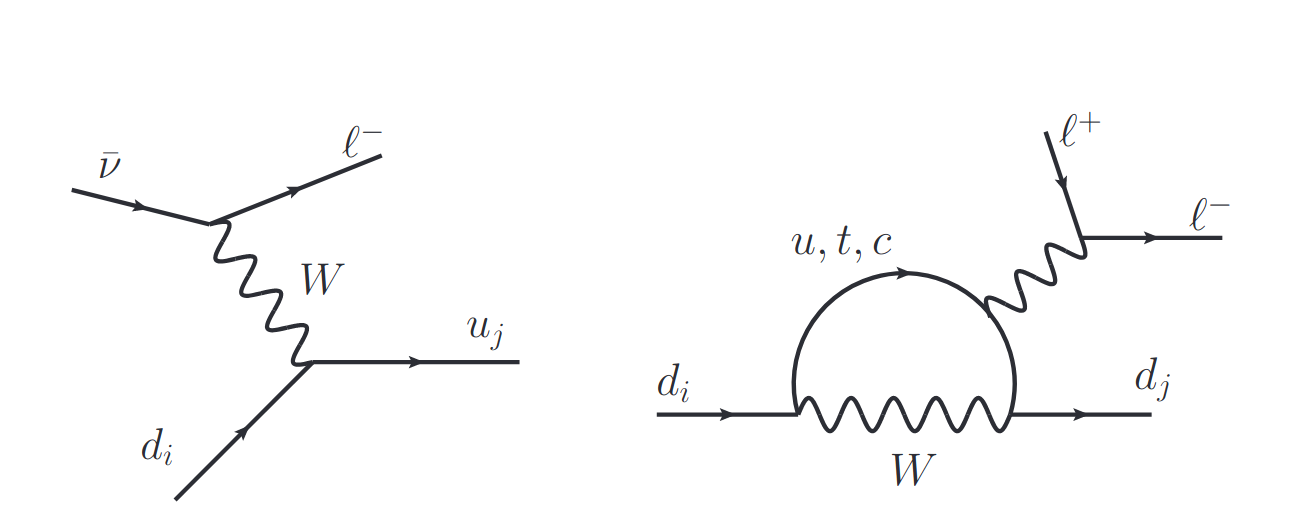
\includegraphics[width=0.75\textwidth]{Stolen.png}
	\caption{Representative tree level charged current diagram (left) and a loop induced FCNC diagram (right).}
	\label{fig:Flavour_D_1}
\end{figure}
%
Make FCNCs a mostly virtual process. Furthermore, the FCNCs come suppressed by the difference of the masses of the quarks running in the loop, $m^2_j-m^2_i$. This so called Glashow-Iliopoulos-Maiani (GIM) mechanism \cite{glashow1970weak}. Given the diferences between the masses of the up and down sectors it has a significant impact. A interesting result would be that that there is no flavour violation, if all the quark masses are the same.

\subsubsection{Flavour as a Probe into New Physics}

Now that we have introduced without great detail flavour physics we can briefly touch on why collider experiments have been sold a as a pathway to discovering new physics i.e. how deviation in rare decays could pin point exactly what is missing in the Standard Model. 

Thanks to these large experiments we have many new observables in flavour physics, e.g. the branching ratios, asymmetries, distributions. There is also a plethora of different parent particles for each change of flavour, as well as many instances of final states. 
%
The abundance of observables is clearly illustrated by opening the handy Particle Data Group (PDG) book \cite{Tanabashi2018} where even the condensed version, the PDG booklet, clocks out at more than 170 pages of mostly tabled information.

%To shorten the discussion we will focus on the processes that are at present showing deviations from the SM expectations. 

The recipe then, seems simple, identify processes that are rare in the SM and then search for deviations from the SM predictions. However thus far all but two processes are within 2$\sigma$ experimental and theoretical bounds given by the SM. They are the $b \rightarrow s \mu \mu$ and $b \rightarrow c \tau \nu$, these are showing over $ 4 \sigma$ deviations from the their expected value. 
%
Avoiding going in depth into these processes, what this might point us too, by these processes as suppressed the vector-axial processes. For them to be integrated away we get very different, but high, energy scales. There would have to exist terms a kin to, 
%If examined through V-A operators the NP scale of these 2 processes are both very different and very heavy, these would be something a kin to, 
%
\begin{equation}
\mathcal{L}_{NP} \supset \frac{1}{\Lambda_{NP}} (\overline{Q}_i \gamma^\mu \sigma^A Q_j ) (\overline{L}_k \gamma_\mu \sigma^A L_l) 
\end{equation}
%
Representing contact interactions of the type, 
%
\begin{equation}
\begin{fmffile}{feyngraph}
  \begin{fmfgraph*}(80,80)
    \fmfstraight
    \fmfleft{i1,i2}
    \fmfright{o1,o2}
    % gluons
    \fmf{gluon}{i1,v}
    \fmf{gluon}{v,i2}
    \fmfblob{200}{v}
    % Higgs boson
    \fmf{gluon}{v,o1}
    \fmf{gluon}{v,o2}
    %\fmf{dashes,tension=1}{v,o1}
    %\fmf{dashes,tension=1}{v,o2}
  \end{fmfgraph*}
\end{fmffile}
\end{equation}
\begin{fmffile}{feyngraph}
  \begin{fmfgraph*}(80,80)
    \fmfstraight
    \fmfleft{i1,i2}
    \fmfright{o1,o2}
    % gluons
    \fmf{gluon}{i1,v}
    \fmf{gluon}{v,i2}
    \fmfblob{20}{v}
    % Higgs boson
    \fmf{dashes,tension=1}{v,o1}
    \fmf{dashes,tension=1}{v,o2}
  \end{fmfgraph*}
\end{fmffile}


To explain $b \rightarrow s \mu \mu$ transitions you would need a $\Lambda_{NP} \approx 3 \ \text{TeV}$ while for $b \rightarrow c \tau \nu$ you would need a $\Lambda_{NP} \approx 30\ \text{TeV}$. This is a strong indicator that some components are missing in our formulation like a new mediator for gauge interactions.  

}

An advantage of the proposed NP scale contributions is that the required scale would avoid most experimental constraints. The FCNC diagram for the particular $b \rightarrow s \mu \mu$ channel can be seen in Fig \ref{fig:Flavour_D_2_Muon}, 

\begin{figure}[H]
	\centering
	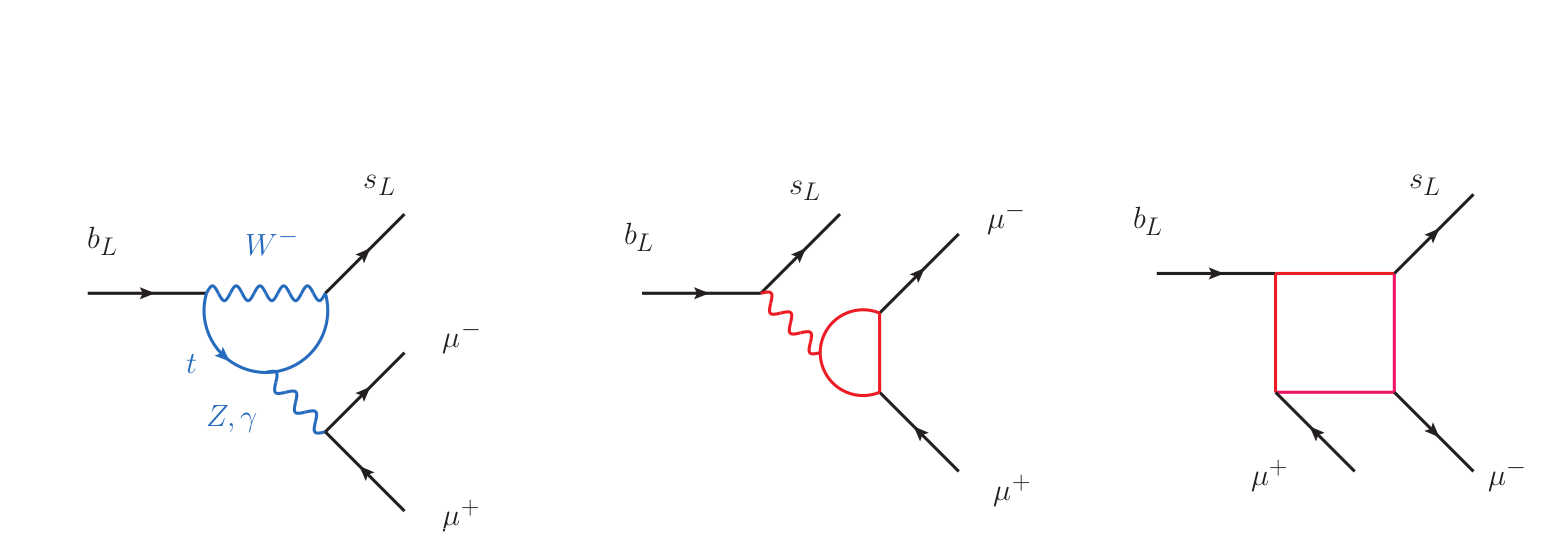
\includegraphics[width=0.75\textwidth]{Stolen_2.png}
	\caption{A representative SM diagram for $b \rightarrow s \mu \mu$ transition (left), and representative possible loop level NP
contributions (middle and right).}
	\label{fig:Flavour_D_2_Muon}
\end{figure}

The $b \rightarrow c \tau \nu$ flavour anomaly is similarly very clean theoretically [
%S. Fajfer, J. F. Kamenik, and I. Nisandzic, Phys. Rev. D85, 094025 (2012), 1203.2654.
], and the disagreement with the
SM predictions is also about 4 $\sigma$. However, the NP effect is large and often this means that the scale of NP needs to be low, and consequently the NP interpretations are often in conflict with the other constraints.

This means the most obvious candidates are ruled out. Theoretical bias would have been that the new charged currents are either due to a charged Higgs, $H^+$ , or a new vector boson, $W^\prime$, see Fig. \ref{fig:Flavour_D_3_Tau}.

\begin{figure}[H]	
	\centering
	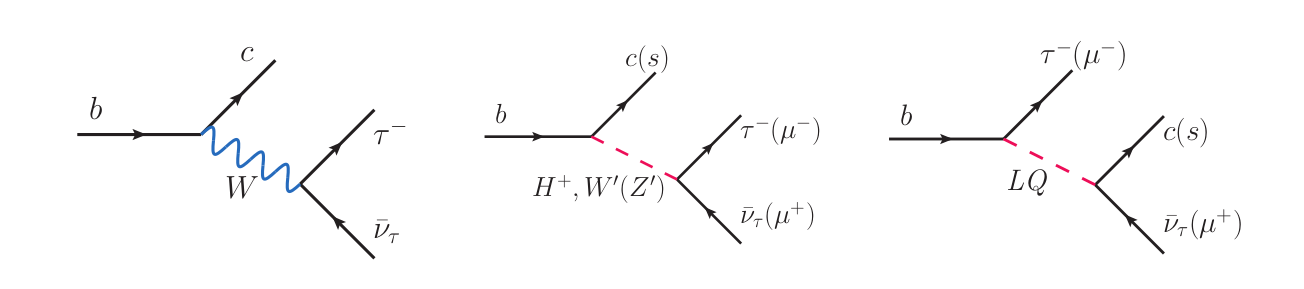
\includegraphics[width=0.75\textwidth]{Stolen_3.png}
	\caption{The SM diagrams for $b \rightarrow c \tau \nu$ transition (left), and the possible tree level NP contributions to $b \rightarrow c \tau \nu$ transition (middle and right).}
	\label{fig:Flavour_D_3_Tau}
\end{figure}

Another prediction of the SM is that the rates for the  $b \rightarrow s e^+ e^-$ and  $b \rightarrow s \mu^- \mu^+$ transitions should be equal to each other. The SM prediction of Lepton Flavour Universality (LFU) is deeply engrained in the structure of the theory, since it is a consequence of the fact that the electroweak gauge group is the same for all three generations. 

The prediction of LFU can be tested experimentally, also trough flavour physics, by theoretically clean observables such as the ratios of these flavour observables, 
%
\begin{equation}
R_{K^{\**}} = \frac{\text{Br}( B \rightarrow K^{\**} \mu^- \mu^+ )}{\text{Br} (  B \rightarrow K^{\**} e^- e^+  )}
\end{equation}
% 
Another strong indicator of new physics is the fact the experimental value for this ratio is $R_{K^{\**}} \approx 0.7$, violating LFU by $2.2 - 2.6 \sigma$

\subsubsection{The Future of Flavour Indirect Searches}

The NP searches with rare decays, as well boost with the upcoming Belle II and LHC upgrades. Belle II expects to collect 50 times the Belle dataset. First collisions were seen in May 2018, and the first B physics run is expected in March 2019. While for the LHC, after upgrade II aims for roughly 100 times the present data set with an upgraded detector. 
%
%A rule of thumb on the improved NP reach gives, for instance for Belle II, that the reach in $\Lambda_NP$ will be improved by $\sqrt[4]{50} \approx 2.7$. Similar if not larger increase applies to LHCb Upgrade II sensitivity improvements. This is a similar jump in energy reach as going from 13 TeV LHC to a 35 TeV LHC!
%
Undoubtedly this improvement in sensibility will translate to a finer value for all measurable parameters at these experiments. We expect these anomalies then to go over the required $5 \sigma$ in future experiments (Assuming of course, they are not statistical deviations). 

{\color{green} 
\section{Quantum chromodynamics}
I should meantion the QCD part of the Lagrangian 

I should explain what is asymptoic freedom and meantion that the strong force fades fast. Free quarks at high energies}


